\documentclass[conference]{IEEEtran}

\usepackage[fleqn]{amsmath}
\usepackage{algpseudocode}
\usepackage{graphicx}
\usepackage{float}
\graphicspath{{images/}}
\interdisplaylinepenalty=2500
\hyphenation{op-tical net-works semi-conduc-tor}

\begin{document}
\title{Parallel Bat Optimization using CUDA}

\author{\IEEEauthorblockN{Jean Carlo Machado}
\IEEEauthorblockA{Universidade do Estado de Santa Catarina\\Master in applied computations\\
UDESC\\
Santa Catarina, Joinville,\\
Email: contato@jeancarlomachado.com.br}
\and
\IEEEauthorblockN{Rafael Stubs Parpinelli}
\IEEEauthorblockA{Univerisdade do Estado de Santa Catarina\\ UDESC\\
Santa Catarina, Joinville
}}

\maketitle

\begin{abstract}
The ever increasing parallel processing power of GPU's is an compelling
reason to implement performance demanding algorithms, like optimization
techniques, using this technology. This work aimed to develop the bat
metaheuristic on GPU and benchmark it against a CPU version. A set of
experiments where conducted in order to measure the speedup difference.
The results suggests that the GPU version is able to achieve relevant
speedups in highly computational demanding problems but for simpler
cases the CPU version might outperform the GPU\@.
\end{abstract}

\IEEEpeerreviewmaketitle
\section{Introduction} %{{{

With the aid of parallel computing, specially GPU computing, it's
possible to tackle ever increasing computational demanding problems in science
with decreasing amounts of time. Further, CPU's are lagging behind GPU's in
many aspects. To give a point of contact, Hwu \cite{programmingProcessors}
mentions that the ratio between many-core GPU's and multi-core CPU's for
peak floating-point calculation throughput is about 10 to 1.

A traditionally complex class of problems are those solved through
the use of meta-heuristics. Within the group of metaheuristics a
special group benefits specially from parallel computing are the swarm
intelligence metaheuristics. Which encompasses many bio-inspirations
like PSO, ACO, and the BAT algorithm. Parpinelli
\cite{newInspirations}, when referring to swarm intelligence algorithms,
define that they are:

\begin{quote} Compounded by a distributed society/population of
individuals where the control is also distributed among the individuals
(there is no centralized control); and the individuals decision-making
is stochastic and based only on local information.\end{quote}

The fact that swarm intelligence algorithms are composed by
independent parts enables them to run in parallel. This work attempts
to investigate the applicability of a relatively new and promising
swarm algorithm: the BAT algorithm using the CUDA model. 

Previously some demonstrations of the bat algorithm parallelized on CPU
were presented in Dao \cite{paralellCPUFirst} and Tsai \cite{paralellCPU}. A
recent publication about the use of the bat optimization on GPU for the training of neural networks can be found on
Choudhdury \cite{firstBatGPU}. However, til the moment of this publications
there's no application of the bat on GPU tested against standard
benchmark functions.

The rest of the paper is organized as following: Section `~\ref{cuda}
gives a overview of CUDA and its components. Section `~\ref{bat}
studies the bat meta-heuristic, it's design and details. Section~\ref{experiments}
details the experiments performed. Section~\ref{results} analyses the results.

%}}}

\section{CUDA} \label{cuda}%{{{

Compute Unified Device Architecture (CUDA) is a general purpose
parallel computing programming model for parallel computations
\cite{cudaDefinition}. CUDA uses a SIMD \textit{single data multiple
execution} approach \cite{gpuOptimization}, where the concurrent code
executes the same instruction but with divergent data.

%%how CUDA is organized?

The basic element of work in a CUDA device is a thread. Groups of
threads are organized in blocks that are themselves wrapped inside
grids. The compute distributor of the GPU allocates this blocks in
Streaming Multiprocessors. Inside the Streaming Multiprocessors the
threads are preferably organized in blocks of 32, called a warp, that
executes at the same time.

\begin{figure}[H]
    \begin{center}
    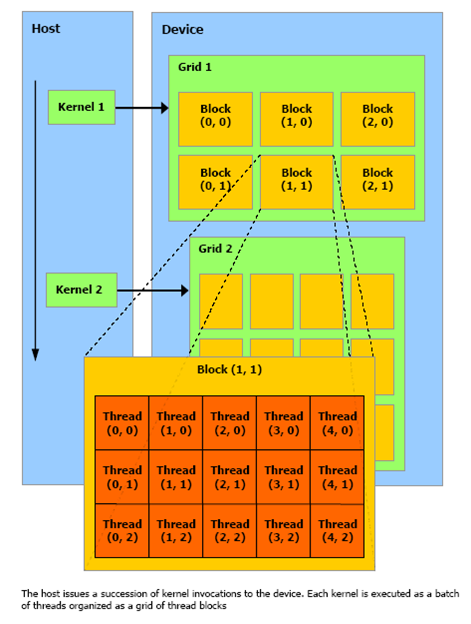
\includegraphics[width=200px,height=200px]{cudaModel}
    \end{center}
    \caption{The CUDA structural organization}
    \label{cuda-organization}
\end{figure}

%%how is CUDA execution model

A CUDA program starts by allocating resources on the GPU (the host)
and dispatching work to be done on the GPU (the device). Once the GPU
finishes it's work, the results are moved back from GPU memory to the
CPU memory. And the results can be returned or further processed.

For the developer, the basic element of concern is the kernel, which is
the function executed on the GPU\@. A kernel function defines the code
to be executed by each of the massive numbers of threads to be invoked
\cite{gpuOptimization}.

Figure~\ref{cuda-organization} illustrates the CUDA architecture mentioned above.

%% some concerns of optimizing applications in CUDA
\subsection{Performance concerns in CUDA}
Since the CUDA model is complex, it's no trivial to setup an ideal configuration 
of a problem in the GPU\@. However many good practises exists and great speedup is already
reported.  Previous researches suggests that highly parallel
applications may speedup up to 450 times \cite{gpuOptimization}.

Below are described some of the major concerns a developer must have
while developing parallel algorithms in CUDA.

\begin{itemize}
    \item When attempting to achieve an application's maximum performance, the primary concern often is managing global memory latency \cite{gpuOptimization}. It's preferable to use local memory and shared memory instead of global since they are much faster.
    \item The less the messaging passing between the GPU and the CPU, the better.
    \item In order to get optimal efficiency the division of work should be in multiples of 32 threads. The hardware will not coalesce threads from different warps \cite{cuda_internals}.
\end{itemize}

%}}}

\section{Bat algorithm} \label{bat} %{{{

The bat algorithm is a populational meta-heuristic introduced by Yang \cite{original} in
2010. It uses the inspiration of micro-bats which uses a type of sonar,
called echolocation, to detect prey, avoid obstacles, and locate their
roosting crevices in the dark \cite{original}.

The bat algorithm is increasingly popular and many successful problems
where solved though it. Induja \cite{bat-usage} mentions some:

\begin{itemize}
\item Clustering
\item Scheduling
\item Phishing detection
\item Document de-duplication
\item Engine rotation tuning
\item Image processing
\end{itemize}


The bat algorithm has two parameters: the pulse rate and the loudness.
As time goes by the pulse-rate tends to increase and the loudness to
decrease. The inspiration comes from the behavior of some bats that use
 slow and loud pitches while in search for a prey and quick
and low pitches when in persecution of one. In the bat algorithm the
loudness is used as a way of accepting bad results (diversification) and
pulse rate as a way of selecting local search (exploitation).

As the base algorithm for our tests we used the bat as proposed by
Cordeiro \cite{comparisonBatParpinelli}. Since this paper has a more detailed
implementation than the original one. The algorithm can be found in Figure~\ref{cpu-pseudo}.

\begin{figure}[H]
\begin{algorithmic}[1]
\State $Parameters:\ n,\alpha,\ \lambda$
\State $initialize\ bats$
\State $evaluate\ fitness$
\State $selects\ best\ \vec{x}_*$
\While {$stop\ criteria\ false$}
    \For{$each\ bat$}
        \State $f_i=f_{min} + (f_{max} - f_{min})\beta, \in \beta [0,1]$
        \State $\vec{v}_i^{t+1} = \vec{v}_i^{t} + (\vec{x}_i^{t} + \vec{x}_*^{t})f_i$
        \State $\vec{x}_{temp} = \vec{x}_i^{t} + \vec{v}_i^{t+1}$
        \If {$rand < r_i, rand \in [0,1] $}
            \State $\vec{x}_{temp} = \vec{x}_* + \epsilon A_m, \epsilon \in [-1, 1]$
        \EndIf

        \State $single\ dimension\ perturbation\ in\ x_{temp}$
        \If {$a < A_i^t\ \textbf{or}\ f(\vec{x}_{temp}) \leq f(\vec{x}_i), a \in [0,1] $}
            \State $\vec{x}_i^t = \vec{x}_{temp}$
            \State $r_i = exp(\lambda * i)$
            \State $A_i =  A_{0} * \alpha^i$
        \EndIf
    \EndFor
    \State $selects\ best\ \vec{x}_*$
\EndWhile
\end{algorithmic}
\caption{Pseudo-code CPU}\label{cpu-pseudo}
\end{figure}

Although some distinctions of the original paper are worth noticing as listed below.

The selection of new results on the original paper tends to be more
greedy. On the original paper, for accepting new results on each
iteration, the loudness must be greater than a aleatory number and the
fitness of the candidate must be better than the current best.
However on the version proposed by Cordeiro \cite{comparisonBatParpinelli} its used
an \textit{OR} operator, so more candidates are accepted (line 14)~\ref{cpu-pseudo}.
The \textit{OR} operator tends to provide more diversity.

Another divergent aspect of the alternative bat is that
it contains a distortion of a single dimension of the results, in order 
to further increase the diversity.

At last, the random algorithm used was not present in neither the
papers. Initially we used the MTGP32 algorithm. However, later was
discovered it's not recommended to use more than 256 threads per block
with it \cite{curandIssue}. So we opted for the XORWOR which has no
limitations of numbers of threads per block.


\subsection{Bat Design on GPU}

\begin{figure}[H]
    \begin{center}
    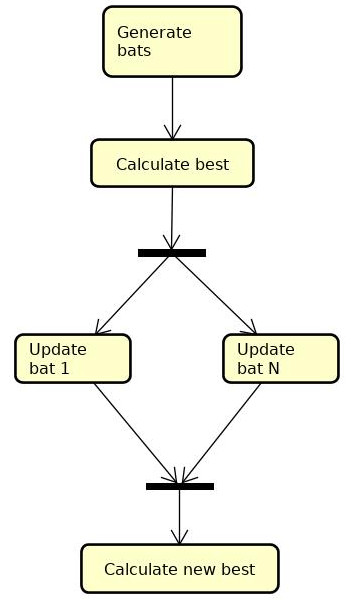
\includegraphics[width=150px,height=200px]{activity}
    \end{center}
    \caption{GPU process flow}
    \label{processFlow}
\end{figure}

A convenient approach to model the swarm in the GPU is to use each
thread as an individual in a single block. Souza \cite{pso-gpu} used a similar method for
a GPU implementation for the PSO algorithm. And, when discussing the
architectural trade-offs of the thread as individual approach, he says:
"allows efficient data parallelism without risk of starvation or race
conditions".

Further, the threaded as individual approach is simple and intuitive.
Allows efficient data sharing through shared memory, making no use of global memory.
The message passing between the CPU and the GPU is kept to the bare minimum as well.
In our implementation there's only the initialization of the device and
the reply to the host with the processed data.


As a drawback of this design is the hardware limitation for working
on a single block. In our GPU the maximum of threads per block is 768
and the memory limit is 16KB\@. Nevertheless neither of this constraints
were limitations on our simulations. While using 768 individuals in ten
thousand iterations with a thousand dimension the memory maximum was
never reached. Either way, it may be a problem when huge amounts of data
are required. Figure~\ref{gpu-pseudo} contains the bat pseudo-code with
the proper changes for working on the GPU\@. Figure~\ref{processFlow}
presents a bigger view of the architecture.

\begin{figure}[H]
\begin{algorithmic}[1]
\State $Parameters:\ n,\alpha,\ \lambda$
\State $initialize\ bats\ asynchronously$
\State $evaluate\ fitness$
\State $synchronize\ threads$
\State $selects\ best\ \vec{x}_*$
\While {$stop\ criteria\ false$}
    \For{$each\ thread$}
        \State $f_i=f_{min} + (f_{max} - f_{min})\beta, \in \beta [0,1]$
        \State $\vec{v}_i^{t+1} = \vec{v}_i^{t} + (\vec{x}_i^{t} + \vec{x}_*^{t})f_i$
        \State $\vec{x}_{temp} = \vec{x}_i^{t} + \vec{v}_i^{t+1}$
        \If {$rand < r_i, rand \in [0,1] $}
            \State $\vec{x}_{temp} = \vec{x}_* + \epsilon A_m, \epsilon \in [-1, 1]$
        \EndIf

        \State $single\ dimension\ perturbation\ in\ x_{temp}$
        \If {$a < A_i^t\ \textbf{or}\ f(\vec{x}_{temp}) \leq f(\vec{x}_i), a \in [0,1] $}
            \State $\vec{x}_i^t = \vec{x}_{temp}$
            \State $r_i = exp(\lambda * i)$
            \State $A_i =  A_{0} * \alpha^i$
        \EndIf
    \EndFor
    \State $synchronize\ threads$
    \State $selects\ best\ \vec{x}_*$
\EndWhile
\end{algorithmic}
\caption{Pseudo-code GPU}
\label{gpu-pseudo}
\end{figure}

%}}}

\section{Experiments} \label{experiments}%{{{

In order to access the performance of the algorithm a set of experiments where
conducted for the following benchmark functions:

\begin{table}[H]
    \renewcommand{\arraystretch}{1.3}
    \caption{Experiments}
    \label{list-of-experiments}
    \centering
    \begin{tabular}{c|c|c|c}
    \hline
        \bf Name & Function &  Dimensions & Agents\\
    \hline
        E1 & Ackley & 100 & 256\\
        E2 & Ackley & 100 & 768\\
        E3 & Griewank & 100 & 256\\
        E4 & Griewank & 100 & 768\\
        E5 & Rastringin & 100 & 256\\
        E6 & Rastringin & 100 & 768\\
        E7 & Rosenbrook & 100 & 256\\
        E8 & Rosenbrook & 100 & 768\\
    \end{tabular}
\end{table}

Each experiment was executed a total of 20 times. A total of 10 thousand
iterations where performed in each experiment. The benchmark functions were
all normalized to work with 100 dimensions for each test. Table~\ref{list-of-experiments}
details each experiment performed.

The experiments were executed on a machine with the following
configuration. A CPU with an Intel(R) Core(TM) i5-4460 CPU @ 3.20GHz. A
GPU GK208 GeForce GT 720 with 1024 MB of vram and a Compute capability
3.5 that belongs to the Kepler architecture (GM10x).


%}}}

\section{Results} \label{results}%{{{

In this section are described the speedup and convergence results.

The fitness of almost all GPU functions presented a slight worse
result when compared with the CPU version. Since there's no noticeable
difference in the design we assume that's related to the way the GPU
process random numbers. Anyway the purpose of this research is to focus
on the speedups so it seems like a reasonable trade-off.

The difference in speedup with a 256 individuals population, when
comparing with the 768's population, shows that as the bat population
increases the performance increases as well on the GPU\@. The contrary is
observed for the CPU.

%cpu
% function & dimensions & population & time_average & time_standard_deviation & fitness_average & fitness_standard_deviation

% ROSENBROOK & 1000 & 128 & 93.2765 & 0.106094 & 12899091640 & 1.11906e+10
% ROSENBROOK & 1000 & 512 & 375.774 & 0.330394 & 999 & 0
% ROSENBROOK & 1000 & 512 & 380.667 & 6.64737 & 2.09486e+09 & 2.96258e+09

%gpu
% ROSENBROOK & 1000 & 128 & 498.714 &  & 1465.49 &
% ROSENBROOK & 1000 & 256 & 406.276 & 6.20077 & 1180.15 & 94.8789
% ROSENBROOK & 1000 & 512 & 125.208 & 0.491476 & 421120 & 21017.6
% ROSENBROOK & 1000 & 512 & 125.433 & 0.0549351 & 432319 & 22367.3
% ROSENBROOK & 1000 & 768 & 138.296 & 0.654157 & 3.41412e+06 & 544668


\begin{table}[H]
    \renewcommand{\arraystretch}{1.3}
    \caption{CPU Results}
    \label{results-cpu}
    \centering
    \begin{tabular}{c|c|c|c}
    \hline
        Time Avg & Time SD & Fit Avg & Fit SD\\
    \hline
        (E1) 49.4428 & 0.0557314 & 4.44089e-16 & 2.05196e-22 \\
        (E2) 161.439 & 0.155131 & 4.44089e-16 & 2.82843e-22 \\
        (E3) 61.3661 & 5.06578   & 0  & 0 \\
        (E4) 162.761 & 57.8119 & 0 & 0 \\
        (E5) 52.0624 & 9.25666   & 0  & 0 \\
        (E6) 171.986 & 14.9089 & 0 & 0 \\
        (E7) 20.4486 & 0.0847218 & 98.9875 & 0.0405622 \\
        (E8) 74.3533 & 0.186482 & 98.9864 & 0.0204378 \\
    \end{tabular}
\end{table}

\begin{table}[H]
    \renewcommand{\arraystretch}{1.3}
    \caption{GPU Results}
    \label{results-gpu}
    \centering
    \begin{tabular}{c|c|c|c}
    \hline
        Time Avg & Time SD & Fit Avg & Fit SD\\
    \hline
        (E1) 17.2255  & 0.708198 &  12.8881 & 2.40027 \\
        (E2) 10.9591  & 0.23902 & 10.9412 & 3.23942 \\
        (E3) 24.2459  & 0.740923  & 2.04281e-15 & 2.60744e-16 \\
        (E4) 15.0012 & 2.01505e-15 & 2.55402e-16 & 0.0394986 \\
        (E5) 30.4483  & 2.0005    & 0 & 0 \\
        (E6) 14.4247 & 0.0543432 & 0 & 0 \\
        (E7) 28.9867 & 1.24554 & 105.03 & 31.2888 \\
        (E8) 15.4403 & 0.326284 & 101.793 & 140.393 \\
    \end{tabular}
\end{table}

% Figure \ref{convergence_comparisom} demonstrates the convergence difference between
% the GPU and CPU.

% \begin{figure}[H]
%     \begin{center}
%     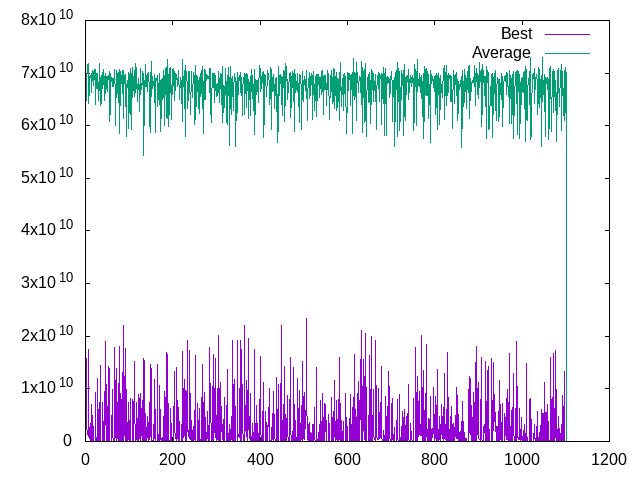
\includegraphics[width=200px,height=200px]{objective}
%     \end{center}
%     \label{convergence_comparisom}
%     \caption{Convergence curves comparison}
% \end{figure}

%}}}

\section{Conclusion} %{{{

With this work it's clear that is possible to speedup the bat
metaheuristic using GPU\@. Notwithstanding the best results are only
achievable on really complex problems with many dimensions.

While working with simpler problems the CPU are a much simpler approach
and may even return better results. However when the problem is so
complex that the time to process is the major issue, the GPU usage
starts to shine. Swarm intelligence metaheuristics are a ideal choice to
apply the parallel architectures due their inner decomposable characteristics.
%}}}

\section{Further works} %{{{

Since the CPU version developed was single threaded it may had some
disadvantages in speedup. The advantages of the algorithm may be tested
against a threaded CPU implementation.

Also, there are hardware constraints that might limit the approach
here proposed. A sub-population approach may serve as an alternative,
considering each GPU block as it's boundaries, somewhat similar to the
work made on parallel bat on CPU by Tsai \cite{paralellCPU}.

%}}}

\begin{thebibliography}{1} %{{{
    \bibitem{original}
    X. S. Yang, "A New Metaheuristic Bat-Inspired Algorithm", in Studies in Computational Intelligence, Sringer Berlin, 284, 2010
\bibitem{comparisonBatParpinelli}
    J.A. Cordeiro and R.S. Parpinelli and H.S. Lopes, "Análise de Sensibilidade dos Parâmetros do Bat Algorithm e Comparação de Desempenho," Department of Bioinformatics, UTFPR
\bibitem{cudaDefinition}
    NVIDIA, "CUDA C Programming Guide," no. July. NVIDIA Corportation, 2013
\bibitem{pso-gpu}
    D. L. Souza et al., "PSO-GPU: Accelerating Particle Swarm Optimization in CUDA-Based
    Graphics Processing Units," in Laboratório de Computação Natural
    (CESUPA)
\bibitem{curandIssue}
    NVIDIA\@.  Bit Generation with the MTGP32 generator [Online]. Available: http://docs.nvidia.com/cuda/curand/device-api-overview.html
\bibitem{paralellCPU}
    C. Tsai, et al. "Parallelized Bat Algorithm with a Communication Strategy," in Modern Advances in Applied Intelligence, 27th International Conference of Industrial Engineering and Other Applications of Applied Intelligent Systems, IEA/AIE 2014
\bibitem{paralellCPUFirst}
    T. Dao et al.,  "Parallel bat algorithm for optimizing makespan in job scheduling problems", in Springer Sience Review, 2015
\bibitem{gpuOptimization}
    S. Ryoo et al.,  "Optimization Principles and Application Performance Evaluation on a Multithreaded GPU using CUDA," in Center of Reliable and High-Performance Computing, University of Illinois
\bibitem{newInspirations}
    Parpinelli, R.S. and Lopes, H.S. (2011) "New inspierations in swarm intelligence: a survey", Int. J. Bio-Inspired Computation, Vol. 3, No. 1 pp.1-16
\bibitem{firstBatGPU}
    A. R. Choudhdury, "A GPU Implementation of a Bat Algorithm Trained Neural Network," in Neural Information Processing 23rd International Conference, ICONIP 2016
\bibitem{programmingProcessors}
    W. W. Hwu and D. Kirk, "Programming massively parallel processors,," in Springer Verlag Gmbh, 2010
\bibitem{bat-usage}
    S. Induja, "Bat Algorithm: An Overview and it's Applicaions,"
    in International Journal of Advanced Research in Computer and Communication Engineering, 2016
\bibitem{cuda_internals}
    How do CUDA blocks/warps/threads map onto CUDA cores? [Online]. Available: http://docs.nvidia.com/cuda/curand/device-api-overview.html

\end{thebibliography}
%}}}
\end{document}
